\chapter{Aspectos Conceituais}
\label{Cap:conceitos}

As técnicas de monitoramento e sensoriamento podem ser usados para as mais diversas funções e implementadas de diversas maneiras. Nesse trabalho, são usadas técnicas, arquiteturas e tecnologias para monitorar o consumo de energia elétrica em um ambiente web monitorada por uma rede de sensores na qual cada sensor da rede transmite seus dados a um componente central que se comunica com essa aplicação em nuvem  \cite{low_cost_wireless_sensor_network_SMF_master_thesis} .

Serão abordados vários conceitos vistos em aula. Um deles engloba o universo dos protocolos e componentes de uma rede sem fio. Isso envolve o estudo do protocolo que será utilizado nesse projeto, que é o ZigBee. Junto a isso são estudados a montagem de circuitos de sensores associados a microcontroladores e a captação dos dados dos sensores por uma central.

Além disso é estudado o desenvolvimento de aplicações para Web e arquitetura de sistemas.

%\section{Circuito AC}
%\label{Sec:ac}

%\todo[inline, color=red!40]{Fazer}


\section{Arquitetura MVC }
\label{Sec:MVC}

A arquitetura de software utilizada é a MVC, composta pelas camadas Model, View e Controller (figura \ref{fig:mvc})\\
\begin{figure}
\centering
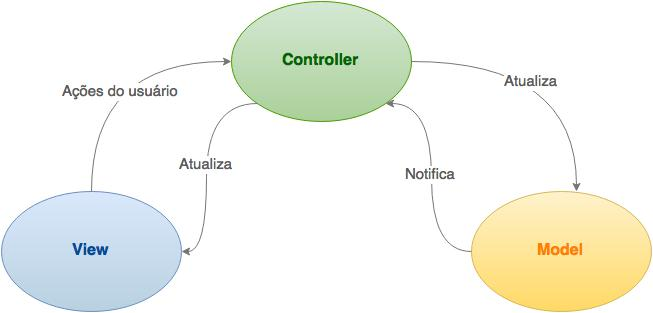
\includegraphics[width=10cm,keepaspectratio]{figuras/MVC.jpg}
\caption{\label{fig:mvc} Arquitetura MVC}
\end{figure}

\textbf{Model:} A camada Model representa a primeira camada de interação com qualquer banco de dados que possa estar sendo usado na aplicação. Ela é responsável por obter, processar, validar dados do banco.\\
\textbf{View:} A view é responsável por usar as informações disponibilizadas para produzir qualquer interface de apresentação que a aplicação pode necessitar.\\
\textbf{Controller:} essa camada lida com as requisições dos usuários. É responsável por se comunicar com a camada Model para realizar operações de busca ou armazenamento de dados e repassar os dados obtidos para a camada View, que irá gerar uma saída resultante para o usuário.\\
MVC é um padrão de projeto de software recomendado para aplicações de desenvolvimento rápido, de fácil manutenção e modular. E foi escolhido como o ideal para um projeto com um tempo limitado de desenvolvimento e possibilita a divisão fácil de tarefas entre os membros da equipe

\section{Wireless Sensor Network }
\label{Sec:WSN}
Wireless Sensor Network, também conhecido como WSN, é um termo genérico que descreve sistemas que tem como objetivo o sensoriamento e monitoração de algum objeto em uma certa área, em pelo menos uma variável (temperatura, humidade, pressão, cor, etc). Os desafios de tais estruturas se resumem a \cite{WSN_survey_JYBMDG_article}: sensores e nós que compõem a rede e podem ter a função de sensoriamento ou de retransmitir dados a um outro nó ou à estação base para serem salvos e devem formar sozinhos uma rede que consiga garantir que os dados sensoriados chegem à base, protocolo de comunicação entre nós, que podem afetar significantemente no consumo de energia, atrasos de comunicação e eficiência do sistema como um todo, fontes de energia dos nós limitada e soluções de coleta de energia. 
%\todo[inline, color=red!40]{Fazer}

\section{Padrão ZigBee e o XBee}
\label{Sec:ZigBee_XBee}
 O padrão ZigBee e o dispositivo XBee possuem muitas características configuráveis e que podem servir a várias aplicações\cite{xbee_book}, porém duas delas são de maior interesse para o trabalho: o baixo consumo de energia e os modos de operação. O XBee pode ser configurado para operar em um dos dois modos: AT ou API. No modos AT há apenas o envio de dados ponto-a-ponto na rede, porém no modo API é possível agir na rede durante sua operação como mudanaças de configuração de nós, broadcast, confirmação de entrega de pacotes e identificação do endereço dos dados recebidos, o que dá ao sistema um maior controle do todo \cite{xbee_documentation}
 
 
\section{Topologias de Rede}
\label{Sec:Redes_topologias}
 Como os nós dos sensores formam uma rede, é necessário analisar as possibilidades de redes.  Como são usados XBees para formar essa rede de sensores, deve-se atentar aos tipos de rede possíveis \cite{xbee_book} \cite{xbee_documentation}.
 
\begin{figure}[H]
\centering
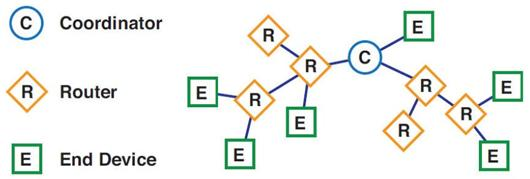
\includegraphics[width=10cm,keepaspectratio]{figuras/zigbee_network_topology.jpg}
\caption{\label{fig:zigbee_network} Topologia de uma rede zigbee}
fonte: \url{http://ftp1.digi.com/support/documentation/html/90001399/90001399_A/Files/XBee-concepts.html}
\end{figure}
 
 A rede ZigBee é composta por nós que podem ser de três tipos:
 \begin{itemize}
\item{Coordenador}: Nó destino (final) de todos os outros nós. Concentra os dados de todos nós. Todas as redes possuem exatamente um nó desse tipo. Não possui a capacidade de dormir e, portanto, não deveria ficar em um dispositivo a bateria limitada. Pode se comunicar com os outros dois tipos de nós. Também não possuem a capacidade de dormir, logo não podem ser energizados com uma bateria limitada. Normalmente são usados para extender a área de uma rede;
\item{Roteador}: Funciona apenas como uma ponte intermediária entre os endpoints e o coordenador. Pode se comunicar com todos os outros tipos de nós;
\item{Dispositivos finais}: Nós que são as pontas da rede e que normalmente estão ligados aos sensores. Esses tem a capacidade de dormir e conservar energia enquanto não transmitem e só não conseguem se comunicar com outros nós do mesmo tipo diretamente;

Dado essas especificações e limitações, as redes formadas por esses componentes podem ser de de três tipos \cite{xbee_book}: estrela, árvore ou mesh. Na estrela os dispositivos finais conversam diretamente com o coordenador, na rede mesh os dispositivos finais estão intermediádos por uma malha de roteadores que se organizam para encontrar o melhor caminho de roteadores de um dispositivo final até o coordenador e a árvore é um subcaso da rede mesh onde devido a bloqueios físicos ou distâncias entre os roteadores, a rede acaba por se tornar uma árvore ou um grafo onde o caminho de um dispositivo final até o coordenador praticamente não possui alternativas.

Devido ao tamanho do projeto, não se justificava usar uma topologia muito complexa, uma vez que a rede teria no máximo quatro nós. Logo, nesse trabalho, é usado uma topologia em estrela.
\end{itemize}
%\section{Cloud Computing}
%\label{Sec:cloud_computing}